% Supplement to Evans 6.3.2: expanded boundary localization and derivative recovery.
\Needspace{35mm}
\subsection{Boundary $H^2$ regularity (Evans \S6.3.2, Theorem 4)}
\begin{theorem}\label{thm:6-boundary-h2}
Suppose $\partial U$ is $C^2$, $A\in C^1(\overline U)$,
$b,c\in L^\infty(U)$ and $f\in L^2(U)$. A weak Dirichlet solution
$u\in H^1_0(U)$ belongs to $H^2(U)$ and satisfies
\[
 \|u\|_{H^2(U)}\leq C(\|f\|_2+\|u\|_2).
\]
If the Dirichlet operator is invertible, the last term can be removed.
\end{theorem}
\begin{expandedproof}

\Needspace{45mm}
\PDEAnnotation{正则性估计不等于可解性}{估计以解已经存在为前提。右边保留 $ \|u\|_2 $ 是为容纳有限维齐次核；只有先证明算子可逆，才能用右端独自控制整个解。}
\paragraph{1. A flat boundary permits tangential differences.}
Work first in a half-ball $B^+_r=\{x\in B_r:x_n>0\}$, where the trace of
$u$ is zero on $x_n=0$. Choose a cutoff vanishing near the curved boundary.
For $k<n$, tangential translation preserves the half-space and the zero
trace, so the test
$-\delta_{-h}(\eta^2\delta_hu)$ remains admissible.
The preceding calculation bounds every $u_{ik}$ with $k<n$ in $L^2$
on a smaller half-ball. This includes the mixed normal--tangential
derivatives, since distributional derivatives commute.

\Needspace{45mm}
\PDEAnnotation{法向差商为何失效}{沿边界平移不会越出半空间，也保留零迹；法向平移会穿过边界，测试函数不再合法。因此先求所有带切向指标的导数，最后用方程解出纯法向导数。}
\paragraph{2. Ellipticity recovers the missing derivative.}
Expand the divergence equation in distributions:
\begin{equation}\label{eq:6-normal-recovery}
 a^{nn}u_{nn}
 =-\sum_{(i,j)\ne(n,n)}a^{ij}u_{ij}
   +(b^i-\partial_j a^{ij})u_i+cu-f.
\end{equation}
Every term on the right is in $L^2$ by Step 1.
Because $a^{nn}\geq\theta$, division bounds $u_{nn}$.
One rigorous way to avoid assuming $H^2$ up to the boundary at this
step is to use the already proved interior $H^2$ theorem: the identity
holds almost everywhere away from $x_n=0$, and its right side has
a uniform $L^2$ bound on the whole smaller half-ball.
The resulting $L^2$ function is the distributional derivative
$u_{nn}$ on this open half-ball. No boundary distribution is introduced
because test functions are supported inside it.

\paragraph{3. Flatten a curved boundary without losing coefficients.}
After a rigid motion, write the boundary as $x_n=\gamma(x')$ and set
\[
 y=\Phi(x)=(x',x_n-\gamma(x')),\qquad
 v(y)=u(\Phi^{-1}(y)).
\]
This particular map has determinant one. Writing $J=D\Phi$, the weak
change of variables gives
\[
 \widehat A(y)=J A J^T,\quad
 \widehat b(y)=Jb,\quad
 \widehat c(y)=c,\quad \widehat f(y)=f,
\]
where all right sides are evaluated at $\Phi^{-1}(y)$.
Indeed $D_xu=J^TD_yv$ and $dx=dy$; the same gradient formula holds
for each test function. Further,
\[
 \xi^T\widehat A\xi\geq\theta|J^T\xi|^2
 \geq\theta\|J^{-T}\|^{-2}|\xi|^2.
\]
Bounded $C^2$ coordinate maps preserve the relevant $H^2$ estimates by
the chain rule, including its lower-order terms.
Since $\gamma\in C^2$ and $A\in C^1$, $\widehat A\in C^1$.
The flat argument therefore applies.

\Needspace{45mm}
\PDEAnnotation{拉平边界也要变换算子}{坐标变换后主系数是 $JAJ^T$。此处选用行列式为一的图形变换；一般坐标变换还会出现体积雅可比因子，不能把它漏掉。}
\paragraph{4. Patch the local estimates.}
A finite boundary cover, together with interior patches, yields
$\|u\|_{H^2}\leq C(\|f\|_2+\|u\|_{H^1})$.
For a solution, G{\aa}rding and
$B[u,u]=(f,u)$ imply
$\|Du\|_2^2\leq C(\|f\|_2^2+\|u\|_2^2)$.
This removes the first-order term. At a nonresonant parameter,
Theorem~\ref{thm:6-discrete} removes $\|u\|_2$ as well.
\end{expandedproof}


\par\noindent\begin{minipage}{\linewidth}
\begin{center}
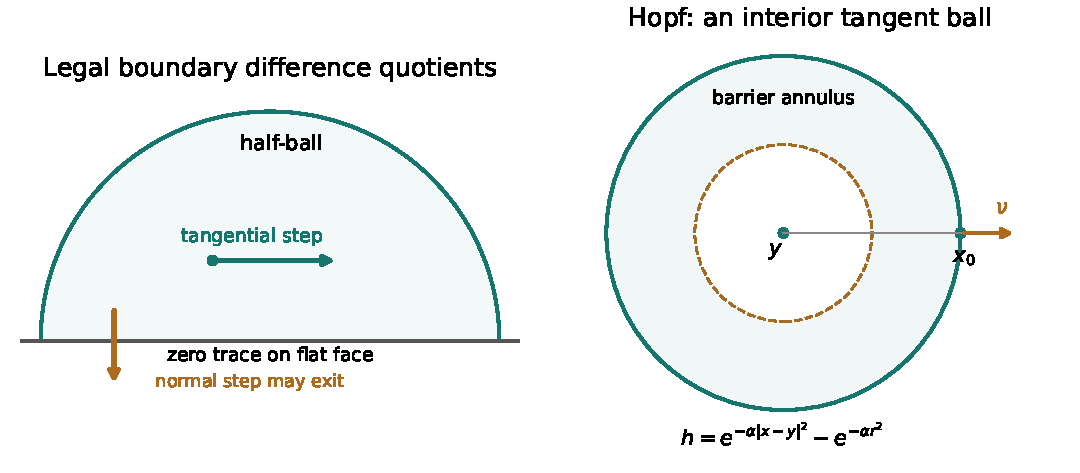
\includegraphics[width=\linewidth]{output/figures/ch06-boundary-tools.pdf}
\end{center}
{\small\textit{Two boundary mechanisms.} Tangential translations preserve
the flat zero-trace face; normal translations need not.
Hopf's exponential barrier is used only in the shaded annulus of an
interior tangent ball. Diagrams are schematic.}
\end{minipage}

\Needspace{35mm}
\subsection{Higher boundary regularity (Evans \S6.3.2, Theorems 5--6)}
\begin{theorem}\label{thm:6-higher-boundary}
If $\partial U$ is $C^{m+2}$, $A,b,c\in C^{m+1}(\overline U)$ and
$f\in H^m(U)$, then a weak zero-Dirichlet solution satisfies
\[
 u\in H^{m+2}(U),\qquad
 \|u\|_{H^{m+2}(U)}
 \leq C\bigl(\|f\|_{H^m(U)}+\|u\|_2\bigr).
\]
Smooth boundary, coefficients and data give $u\in C^\infty(\overline U)$.
\end{theorem}
\begin{expandedproof}
The case $m=0$ is Theorem~\ref{thm:6-boundary-h2}.
For the induction step assume $u\in H^{m+2}$ and $f\in H^{m+1}$,
with coefficients $C^{m+2}$ and boundary $C^{m+3}$.
In a flattened chart, differentiate $m+1$ times only tangentially.
The resulting derivative has zero trace on the flat face, because
tangential differentiation commutes with the trace at these orders.
Its localized equation has an $L^2$ right side: expand the commutators
exactly as in the interior proof. Cutoffs keep tests away from the
curved part of the chart. Applying boundary $H^2$ gives all derivatives
of total order $N=m+3$ having at most two normal differentiations.

Recover the others from \eqref{eq:6-normal-recovery}. To estimate an
order-$N$ derivative with $q\geq3$ normal indices, apply an order-$N-2$
derivative with $q-2$ normal indices to that identity.
The desired term is multiplied by $a^{nn}$; the other order-$N$ terms
have at most $q-1$ normal indices, and coefficient commutators contain
derivatives of $u$ of order at most $N-1$, already controlled.
Induct on $q$ and divide by $a^{nn}\geq\theta$.
These differentiated identities can be justified first by interior
regularity and then by the uniform estimates up to the flat face,
as in the $H^2$ case. Patching proves the global estimate.
Finally extend Sobolev functions across the smooth boundary and use
embedding at arbitrarily high orders to obtain $C^\infty(\overline U)$.
\end{expandedproof}
\Needspace{45mm}
\PDEAnnotation{边界光滑度不能省略}{内部正则性只看系数和右端，边界正则性还看区域形状。角点可能产生奇性；零边界条件本身并不能保证解在角点附近有平方可积的二阶导数。}
\paragraph{What the estimates actually say.}
The two-derivative gain is an a priori estimate for solutions, not an
existence theorem by itself. At an eigenvalue, the term $\|u\|_2$
cannot be removed: a nonzero eigenfunction solves a homogeneous
shifted equation. Nonzero boundary data require a sufficiently regular
lift before the zero-boundary theorem can be used.